\documentclass[12pt]{article}
\usepackage[utf8]{inputenc}
\usepackage{geometry}
\usepackage{graphicx}
\usepackage{parskip}
\usepackage{amsmath}
\usepackage{hyperref}
\usepackage{titlesec}
\usepackage{subcaption}

\geometry{a4paper, margin=1in}

\title{\bf About My Home Town: Development Guide \\ \large CSC478: Software Engineering Capstone}
\author{Audrey Yates, William Morgan, Steven Hogue \\ Group 11}
\date{\today}

\begin{document}

\maketitle

\tableofcontents

\newpage

\section{Requirements Documentation}\label{sec:scope}

\subsection{Introduction}

\subsubsection{Scope}

We will construct a cross-platform web application that allows users to check on a variety of data points for their locale. This data may include, but is not limited to, gas prices, current and forecast weather, restaurant/food prices, public facilities, local businesses, and possibly crime information. The goal is to compile as much data from public or low-cost API's into a single interface, adding statistical analysis, and overlaying it into a mapping application (such as Google Maps). As a long-term goal we would like to interpret and nd news articles relating to an area of interest, and pin the location in which they took place on the map.

\subsubsection{Definitions, Acronyms, and Abbreviations}

\begin{itemize}
    \item \textbf{The Application:} The web application we are building, which will be called "About My Home Town"
    \item \textbf{API:} Application Programming Interface
    \item \textbf{Authenticated User:} A user who has created an account and logged in
    \item \textbf{Bcrypt:} A password hashing function
    \item \textbf{HTTP:} Hypertext Transfer Protocol
    \item \textbf{HTTPS:} Hypertext Transfer Protocol Secure
    \item \textbf{JSON:} JavaScript Object Notation
    \item \textbf{Local Storage:} A method of storing data in the user's browser
    \item \textbf{Non-Authenticated User:} A user who has not logged in
    \item \textbf{RESTful API:} A type of API that follows the REST architectural style
    \item \textbf{Salt:} A random value that is used as an additional input to a one-way function that hashes data
    \item \textbf{Session Token:} A unique token generated when a user logs in, which is used to authenticate the user
    \item \textbf{User:} The end user of the application
    \item \textbf{Widget:} A small unit of data presentation, containing a sample of data we provide (ex. Weather Widget, Restaurant Widget, etc.)
\end{itemize}

\subsection{General Description}

\subsubsection{Product Perspective}

The application we are building will be useful for users who want to access a wide range of data points for their locale in a single interface. This comprehensive approach saves users time and effort by eliminating the need to visit multiple websites or applications to gather this information. By building this application, we are addressing the need for a centralized platform that provides users with a wealth of localized information, ultimately making it easier for them to make informed decisions and navigate their surroundings.

\subsubsection{Product Functions}

This application will aggregate data from various public free and paid sources into a single interface. It will allow users to save their data by logging in and creating an account with their zip code, and then it will show them information regarding their local area, such as weather and restaurant information.

\subsubsection{User Characteristics}

Our prospective users are people who are interested in accessing a range of data points for a given area, such as users looking to move into a new area, users who are traveling, or users who are simply curious about their current surroundings and want to explore. The thing all of these users have in common is that they are looking for a centralized platform that provides them with a wealth of localized information.

\subsubsection{General Constraints}

This has to be built as a web application with constant network access, meaning that it necessarily \textit{cannot} work offline. Due to this, the end user must access our application through a web browser that supports modern JavaScript features.

Another constraint of this is that the data we are pulling in is only as good as the data we are given. If a data source is inaccurate, our application will be inaccurate as well.

\subsubsection{Assumptions and Dependencies}

There are few assumptions from the end user, though as mentioned above, we will assume both that the end user is accessing from a modern web browser and that the data we are pulling in is accurate.

\subsection{Specific Requirements}

\subsubsection{Data Sources (1)}

\setlength{\tabcolsep}{1cm}
\begin{tabular}{|l|p{8cm}|}
    \hline
    Requirement Number & Description                                                                                                          \\

    \hline\hline
    1.0.0              & The application must pull in the most recently available weather data whenever the end user loads the application    \\

    \hline\hline
    1.1.0              & The application must pull in the most recently available restaurant data whenever the end user loads the application \\
    \hline
\end{tabular}

\subsubsection{User Data (2)}

\setlength{\tabcolsep}{1cm}
\begin{tabular}{|l|p{8cm}|}
    \hline
    Requirement Number & Description                                                            \\

    \hline\hline
    2.0.0              & Any user must be allowed to create an account with \bf required fields \\
    \hline
    2.0.1              & Email Address, 45 character string                                     \\
    \hline
    2.0.2              & ZIP Code, either ZIP or ZIP+4 format stored as a string                \\ \hline
    2.0.3              & Password, arbitrary length                                             \\

    \hline\hline
    2.1.0              & Any user must be allowed to create an account with \bf optional fields \\
    \hline
    2.1.1              & First Name, 45 character string                                        \\
    \hline
    2.1.2              & Last Name, 45 character string                                         \\
    \hline
    2.1.2              & Bio Information, 256 character string                                  \\
    \hline
\end{tabular}

\subsubsection{Authentication Model (3)}

\setlength{\tabcolsep}{1cm}
\begin{tabular}{|l|p{8cm}|}
    \hline
    Requirement Number & Description                                                                                          \\

    \hline\hline
    3.0.0              & Email addresses must be globally unique                                                              \\

    \hline\hline
    3.1.0              & Users must be able to log in with their email and password                                           \\

    \hline\hline
    3.2.0              & Passwords must be handled securely in all cases                                                      \\
    \hline
    3.2.1              & Passwords must be at least 6 characters in length                                                    \\
    \hline
    3.2.2              & Passwords must be sent to the server over HTTPS                                                      \\
    \hline
    3.2.3              & Passwords must be encrypted using Bcrypt with a hash on the server side only                         \\
    \hline
    3.2.4              & During user verification, passwords should hashed using the salt, and checked against the known hash \\
    \hline
    3.2.5              & Passwords must \textbf{NEVER} be stored in plaintext, only during transit                            \\

    \hline\hline
    3.3.0              & When a user logs in, a session token should be generated                                             \\
    \hline
    3.3.1              & Session tokens must be stored along with the user's email in the database, and a last used date      \\
    \hline
    3.3.2              & Session tokens must simultaneously be stores in the user's browser's local storage                   \\
    \hline
    3.3.4              & To authenticate a user's existing session, the local token must be one of the known session tokens   \\
    \hline
    3.3.5              & If a token is older than 24 hours, invalidate it and force log out the user                          \\

    \hline\hline
    3.4.0              & Users must be able to log out of their account, invalidating the session                             \\
    \hline
\end{tabular}

\subsubsection{User Interface (4)}

\setlength{\tabcolsep}{1cm}
\begin{tabular}{|l|p{8cm}|}
    \hline
    Requirement Number & Description                                                                                                     \\

    \hline\hline
    4.0.0              & The application must have an intuitive user interface                                                           \\

    \hline\hline
    4.1.0              & The application must have a home page                                                                           \\
    \hline
    4.1.1              & This page must be available to only authenticated users                                                         \\
    \hline
    4.1.2              & This page must show an overview of the data we present in other locations on the site in widgets                \\

    \hline\hline
    4.2.0              & The application must have an about page                                                                         \\
    \hline
    4.2.1              & This page must be available to all users                                                                        \\
    \hline
    4.2.2              & This page must show a description of the site and its technology                                                \\
    \hline

    \hline\hline
    4.3.0              & The application must have a sign up page                                                                        \\
    \hline
    4.3.1              & This page must be available to only \textit{non} authenticated users                                            \\
    \hline
    4.3.2              & This page must allow the user to create an account based on the User Data and Authentication Model requirements \\
    \hline

    \hline\hline
    4.4.0              & The application must have a sign in page                                                                        \\
    \hline
    4.4.1              & This page must be available to only \textit{non} authenticated users                                            \\
    \hline
    4.4.2              & This page must allow the user to sign in based on the User Data and Authentication Model requirements           \\
    \hline
    4.4.2              & After a user has signed in, they are now considered authenticated                                               \\
    \hline

    \hline\hline
    4.5.0              & The application must have a sign out button                                                                     \\
    \hline
    4.5.1              & This button must be visible to only authenticated users                                                         \\
    \hline
    4.5.2              & This page must allow the user to sign out, invalidating their session                                           \\
    \hline
    4.5.2              & After a user has signed out, they are again considered non-authenticated                                        \\
    \hline

    \hline\hline
    4.6.0              & The application must have a user modification page                                                              \\
    \hline
    4.6.1              & This page must be available to only authenticated users                                                         \\
    \hline
    4.6.2              & This page must allow the user to modify any of their user data (with exception to the password and email)       \\
    \hline
    4.6.2              & After submitting modifications, all data must update immediately and the page should refresh                    \\
    \hline
\end{tabular}

\subsubsection{User API (5)}

\setlength{\tabcolsep}{1cm}
\begin{tabular}{|l|p{8cm}|}
    \hline
    Requirement Number & Description                                                                                                           \\

    \hline\hline
    5.0.0              & The application must have a RESTful API that allows for the creation, reading, updating, and deletion of user data    \\

    \hline\hline
    5.1.0              & This API must be available at the 'api' subdomain of the application site                                             \\

    \hline\hline
    5.2.0              & All API specifications must return the User object as JSON on a succesful result, otherwise return an HTTP error code \\

    \hline\hline
    5.3.0              & The API must include an endpoint to allow user creation (sign up)                                                     \\

    \hline\hline
    5.4.0              & The API must include an endpoint to allow user authentication (sign in)                                               \\

    \hline\hline
    5.5.0              & The API must include an endpoint to allow sesion token validation                                                     \\

    \hline\hline
    5.6.0              & The API must include an endpoint to allow the user modification (update user)                                         \\

    \hline
\end{tabular}

\newpage

\section{Design Documentation}

The following design elements were composed prior to any work on the application, and should generally be followed throughout the development process.

\subsection{Architecture Diagrams}

This diagram shows the layout of the AWS architecture we are using for our application. The user interacts with the CloudFront Distribution, which then sends the request to the S3 bucket. The S3 bucket then returns the static template for the site to the end user.

From there, the user's browser interacts with the API Gateway, which then sends the request to the Lambda function. The Lambda function then interacts with the DynamoDB database to get or set the user's data. If no live data is available, the Lambda function will then interact with the external API to get the data.

\begin{figure}[htbp]
    \centering
    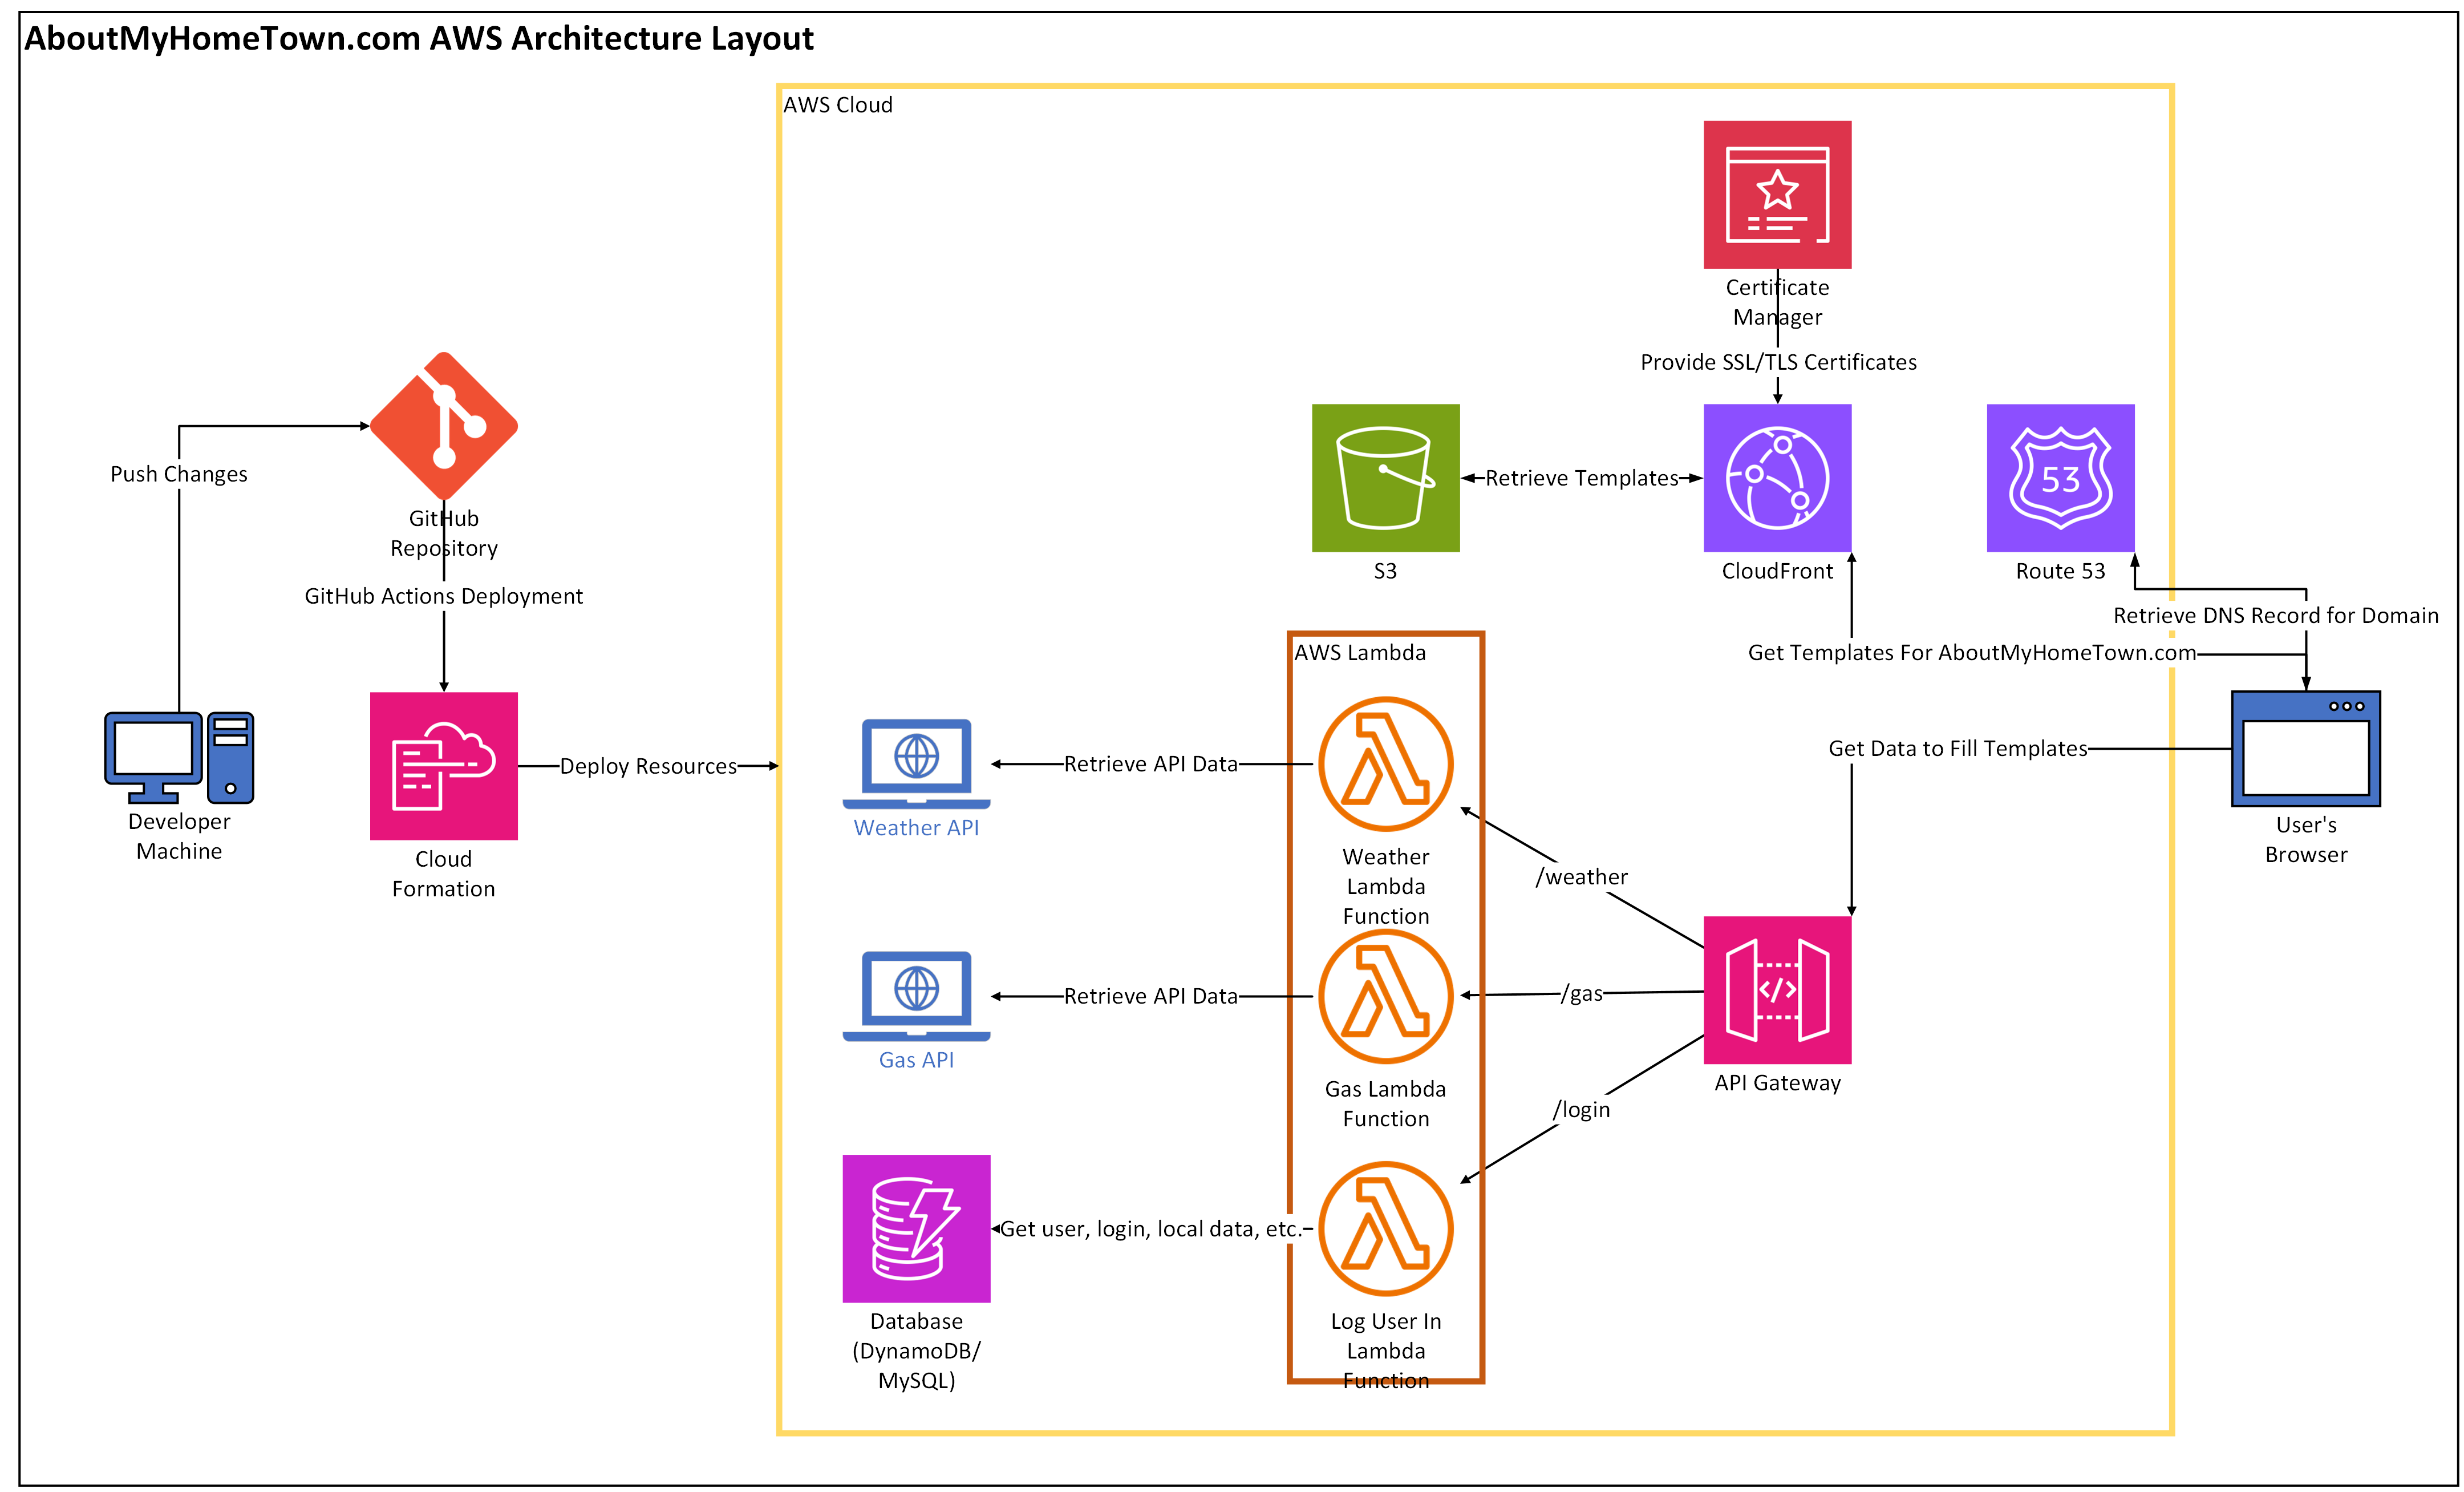
\includegraphics[width=\textwidth]{images/aws_architecture_layout.png}
    \caption{AWS Architecture Layout}
    \label{fig:architecture}
\end{figure}

\subsection{Wireframes}

\begin{figure}[htbp]
    \begin{subfigure}[b]{0.48\textwidth}
        \centering
        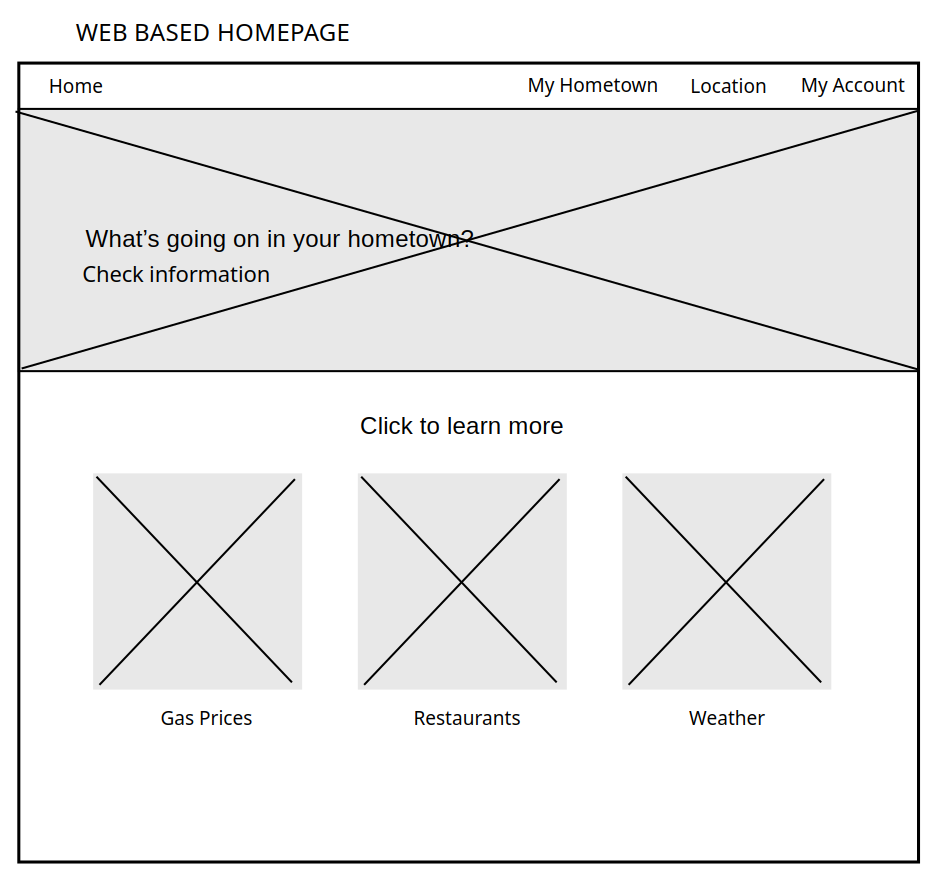
\includegraphics[width=\textwidth]{images/homepage.png}
        \caption{Home Page}
    \end{subfigure}
    \hfill
    \begin{subfigure}[b]{0.48\textwidth}
        \centering
        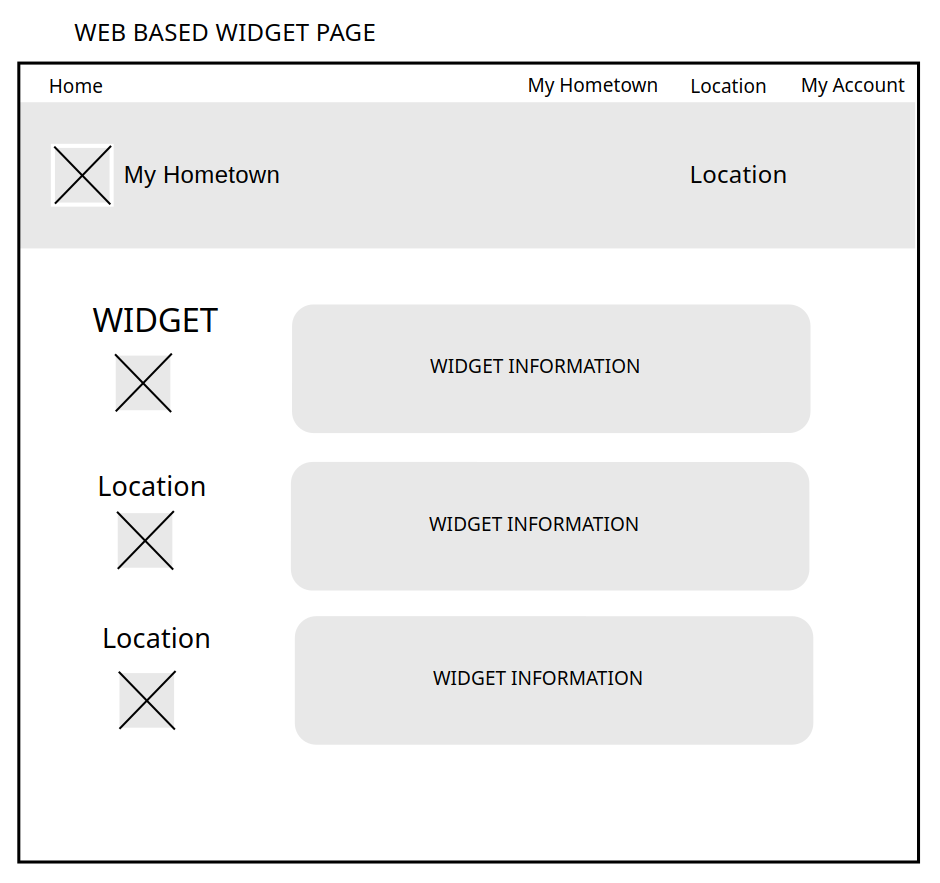
\includegraphics[width=\textwidth]{images/widgets_page.png}
        \caption{Widgets Page}
    \end{subfigure}
    \centering
    \begin{subfigure}[b]{0.48\textwidth}
        \centering
        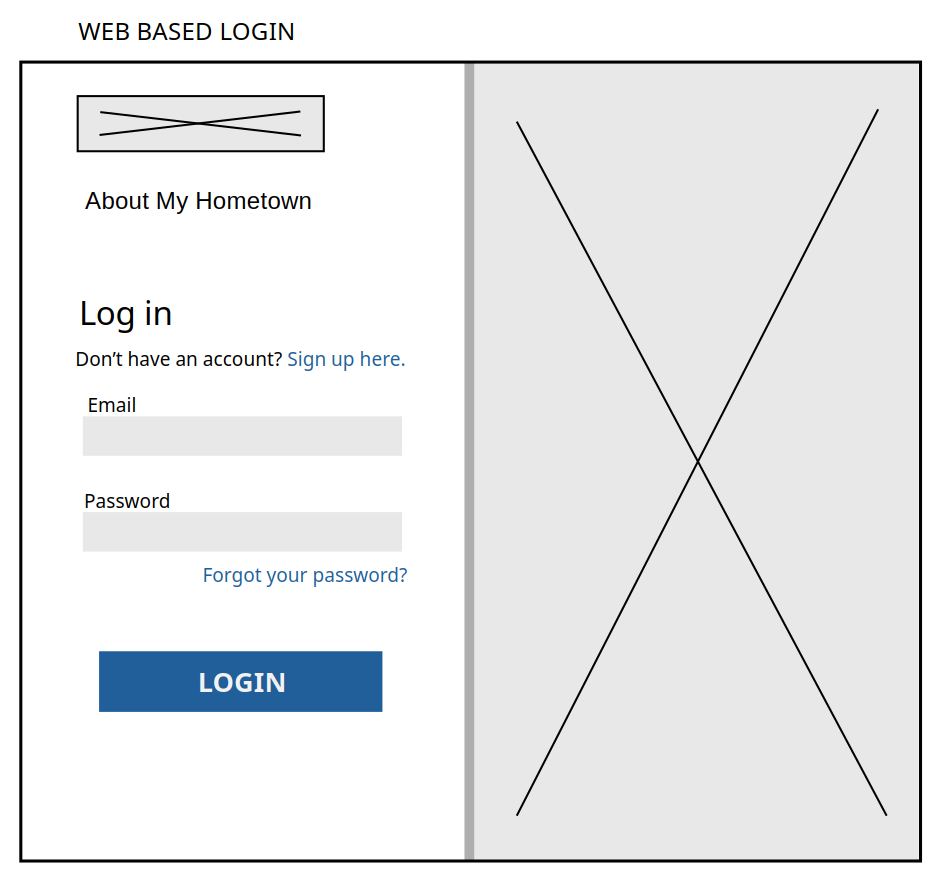
\includegraphics[width=\textwidth]{images/sign_in_page.png}
        \caption{Another Page}
    \end{subfigure}
\end{figure}

This figure shows the initial wireframed designs for our sign in page, homepage, and widgets page. We added to these designs, but the overall design philosophy remained the same.

\newpage

\section{Testing Documentation}

\textbf{Note:} for all testing, you need to completely set up your environment. This means running at least:
\begin{verbatim}
    npm install
\end{verbatim}

\subsection{End to End Testing}

This application supports full end to end testing of the application completely locally on the developer's machine. This is done in a few stages, with each stage representing a different part of the infrastructure.

Regardless of how you decide to test, if you follow either guide to set up the application listed below, you can access the application at \url{http://localhost:4200}. This allows the developer to see the application as the end user would see it, while having the ability to immediately test and see any changes they make.

\subsubsection{Piece by Piece}
\begin{itemize}
    \item \textbf{Frontend:} The frontend is tested using the Angular CLI. The following will start the Angular CLI locally:

          \begin{verbatim}
    ng serve --open --watch --port 4200
          \end{verbatim}

          Once the Angular CLI is running, you can access the application at \url{http://localhost:4200}.

    \item \textbf{Database:} The database is tested by spinning up a MySQL Docker container. The following will start the MySQL container:

          \begin{verbatim}
    docker run --name my-local-mysql \\
        -e MYSQL_ROOT_PASSWORD=localpass \\
        -e MYSQL_DATABASE=mydb -p 3306:3306 -d mysql:latest \\
        --default-authentication-plugin=mysql_native_password
        \end{verbatim}

          This will start a \textit{local and not-for-production} MySQL container with the root password set to 'localpass', the database name set to 'mydb', and the container will be accessible on port 3306.

    \item \textbf{Backend:} The backend is tested using the AWS SAM CLI. The following will start the SAM API locally:

          \begin{verbatim}
    cd aboutmyhometown-lambda-stack
    sam local start-api -p 4201
          \end{verbatim}

          Once the SAM API is running, you can access the API at \url{http://localhost:4201}.
\end{itemize}

\subsubsection{Helpers}

While you can test the application piece by piece, we have set up a much simpler way to test. The following will start the entire application locally all at once, handling seting up and tearing down the database, and starting the frontend and backend:

\begin{verbatim}
    npm run start-all
\end{verbatim}

Or, for Linux users:

\begin{verbatim}
    npm run start-all-linux
\end{verbatim}

\subsection{AWS CloudFormation Testing}

The AWS infrastructure deployed from this repository (the API Gateway and Lambda functions) can be tested using the AWS SAM CLI as well. The following command can be used to validate that the templates are valid configurations:

\begin{verbatim}
    sam validate -t aboutmyhometown-lambda-stack/template.yaml
\end{verbatim}

\subsection{Unit Testing}

\setlength{\tabcolsep}{3mm}
\begin{tabular}{|c|c|l|l|l|}
    \hline
    Test & Requirement & Rationale & Input   & Expected \\

    \hline
    1    & 1.0.0       & Example   & Example & Example  \\
    \hline
\end{tabular}



\newpage

\section{Known Bugs}

\begin{itemize}
    \item We were unable to get the HTTPS version of the redirect to 'www.' to work properly
          \begin{itemize}
              \item Any of the following redirect properly to the main site:
                    \begin{itemize}
                        \item \url{http://aboutmyhometown.com}
                        \item \url{http://www.aboutmyhometown.com}
                        \item \url{https://www.aboutmyhometown.com}
                    \end{itemize}
              \item However, the following does not redirect properly:
                    \begin{itemize}
                        \item \url{https://aboutmyhometown.com}
                    \end{itemize}
              \item This seems to be a technology issue with the way S3 redirects, and it is unable to redirect HTTPS traffic without configuring a secondary route through the CloudFront Distribution
          \end{itemize}
\end{itemize}

\end{document}
